\section*{Test 12 Effect of bottlenecks}

Construct a room that is connected to another room by a corridor and fill it as illustrated with a population of 150 adults (walking speed accordance with Figure 5). The premovement time is 0 s.

\noindent
As the flow of persons through the corridor is limited, congestion should only occur in room 1 and not in room 2.


\begin{figure}[h]
	\centering
	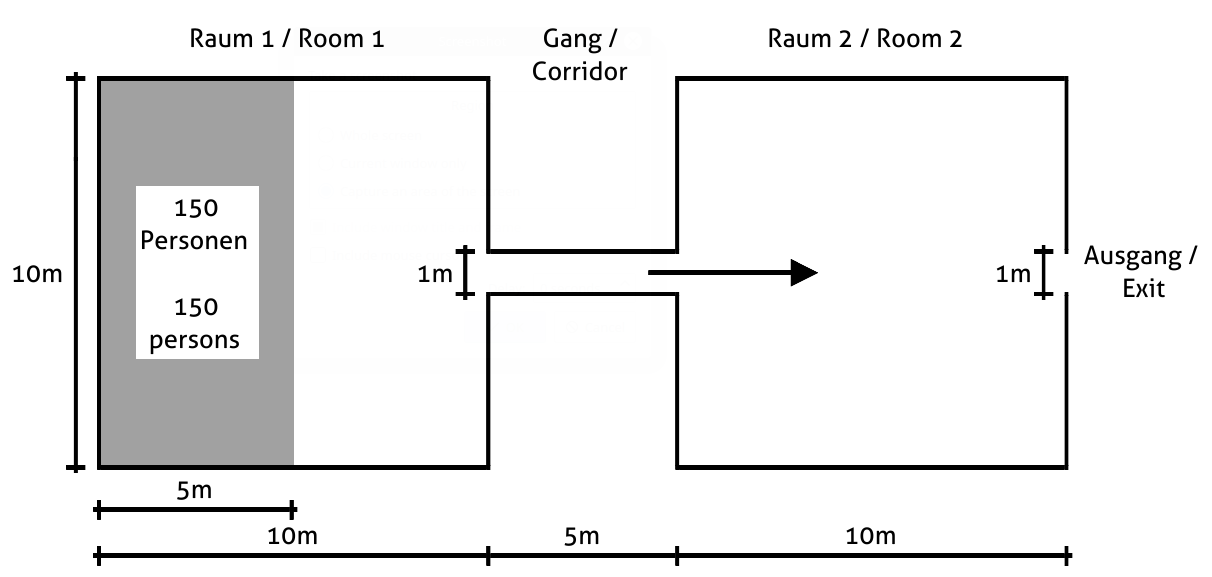
\includegraphics[scale=0.44]{test_description/Corridor_test_12.png}
	\caption{\footnotesize \textbf{The effect of the bottleneck leads to the formation of congestion in front of the corridor which means congestion in front of the exit is avoided.
}}
\end{figure}

\noindent
As long as no decision can be made on an empirical basis on whether congestion can in fact occur at the entrance to room 2, test 12 should not be treated as an exclusion criterion and should only document model behaviour.
